\documentclass[11pt]{article}
\usepackage{algorithm2e}
\usepackage[italian]{babel}
\usepackage[document]{ragged2e}
\usepackage{amsfonts, amssymb, amsmath}
\usepackage{cancel}
\usepackage{float}
\usepackage{mathtools}
\usepackage[margin=3cm]{geometry}
\usepackage{subfig}
\usepackage{mwe}
\usepackage{hyperref}

\tolerance=1
\emergencystretch=\maxdimen
\hyphenpenalty=10000
\hbadness=10000

\begin{document}
\graphicspath{ {./img/} }
\begin{titlepage}
    \begin{center}
        \vspace*{1.5cm}
            
        \Huge
        \textbf{IMAGING} \\
        \LARGE
        Deblur
            
        \vspace{0.5cm}
        \LARGE
        Relazione
            
        \vspace{1.5cm}
          
        \begin{minipage}[t]{0.47\textwidth}
        \begin{center}
        	{\large{\bf Cheikh Ibrahim $\cdot$ Zaid}}\\
			{\large Matricola: \texttt{0000974909}}
        \end{center}

		\end{minipage}
		\hfill
		\begin{minipage}[t]{0.47\textwidth}\raggedleft
		\begin{center}
        	{\large{\bf Xia $\cdot$ Tian Cheng}}\\
			{\large Matricola: \texttt{0000975129}}
        \end{center}
		\end{minipage}  
            
        \vspace{6cm}
            
        Anno accademico\\
        $2021 - 2022$
            
        \vspace{0.8cm}
            
            
        \Large
        Corso di Calcolo Numerico\\
        Alma Mater Studiorum $\cdot$ Università di Bologna\\
            
    \end{center}
\end{titlepage}
\pagebreak

\section{Introduzione}
Il progetto consiste nel ricostruire un'immagine a partire da una sua istanza alterata da uno sfocamento noto e un rumore casuale.\\
Si tratta di un problema solitamente affrontato elaborando immagini provenienti da un dispositivo di acquisizione che nel suo processo di cattura deve digitalizzare un segnale analogico.\\ 
La soluzione di tale problema viene formulata come problema ai minimi quadrati:
\begin{align*}
    \min\limits_{x} \frac{1}{2} \Vert Ax-b \|_{2}^{2}
\end{align*}
dove $A$ è l'operatore di blur, $x$ l'immagine ricostruita e $b$ l'immagine acquisita.\\
Per la risoluzione sono note diverse formulazioni. Quelle impiegate sono:
\begin{itemize}
    \setlength\itemsep{0.05cm}
    \item Metodo naive $\min\limits_{x} \frac{1}{2} \Vert Ax-b \|_{2}^{2}$. Questo approccio è noto essere mal condizionato.
    \item Regolarizzazione di Tikhonov $\min\limits_{x} \frac{1}{2} \Vert Ax-b \|_{2}^{2} + \lambda \Vert x \|_{2}^{2}$
    \item Regolarizzazione tramite variazione totale $\min\limits_{x} \frac{1}{2} \Vert Ax-b \|_{2}^{2} + \lambda \phi_{\text{TV}}(x)$
\end{itemize}
Per misurare la qualità dei risultati verranno impiegate due metriche:
\begin{itemize}
    \setlength\itemsep{0.05cm}
    \item Mean Squared Error (MSE) \textbf{[AGGIUNGERE DESCRIZIONE]}
    \item Peak Signal-to-Noise Ratio (PSNR) \textbf{[AGGIUNGERE DESCRIZIONE]}
\end{itemize}

\newpage
\section{Esecuzione preliminare}
\label{chap:lambda}
Per avere una visione sul comportamento delle varie formulazioni, è stata eseguita una prima sperimentazione sull'immagine in \autoref{fig:originale1}
\begin{figure}[H]
    \centering
    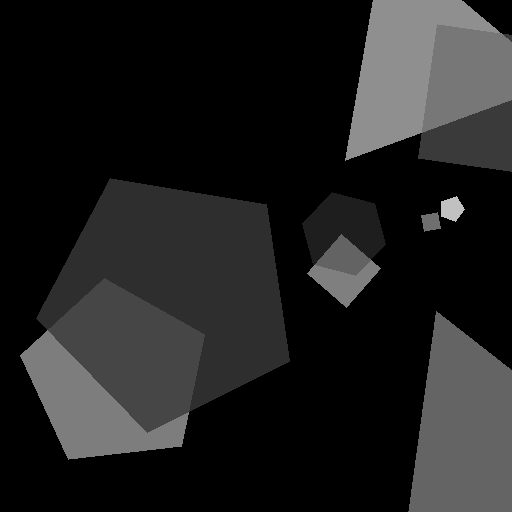
\includegraphics[width=4cm]{esecuzione/originale.png}
    \caption{Immagine di test}
    \label{fig:originale1}
\end{figure}

\subsection{Prima esecuzione}
La prima esecuzione è stata eseguita con un blur generato da un kernel $5 \times 5$ con $\sigma=0.5$ e rumore gaussiano con deviazione standard $0.05$.

\subsubsection{Stima di $\lambda$}
Per eseguire i metodi regolarizzati è necessario prima determinare il valore $\lambda$ del parametro di regolarizzazione.\\
Esistono condizioni che permettono di determinare se un valore di $\lambda$ sia accettabile o meno. In questo progetto verrà determinato utilizzando una ricerca iterativa del punto migliore.\\
Il seguente grafico mostra il valore del PSNR al variare di $\lambda \in [0.01, 1]$ con passo $0.01$ per Tikhonov:
\begin{figure}[H]
    \centering
    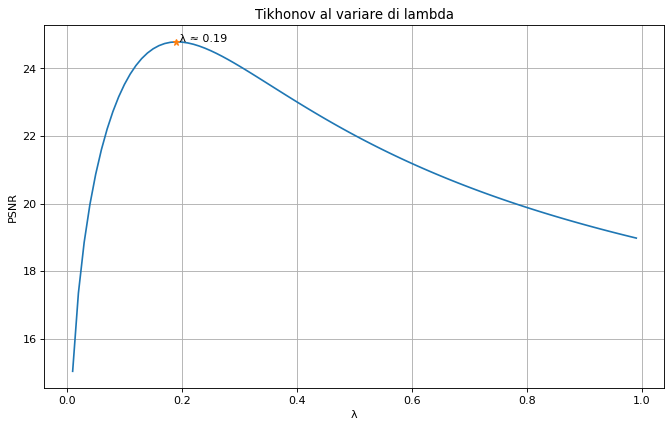
\includegraphics[width=10cm]{esecuzione/1/tikhonov_lambda.png}
    \caption{$\lambda=0.19$ e $\texttt{PSNR} \simeq 24.79$}
    \label{fig:tikhonov_lambda1}
\end{figure}
Analogamente, il seguente grafico mostra la variazione del PSNR per $\lambda \in [0.01, 1]$ con passo $0.01$ per la variazione totale:
\begin{figure}[H]
    \centering
    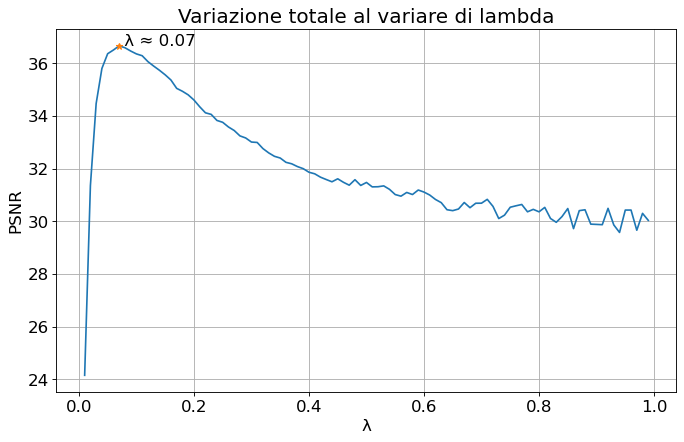
\includegraphics[width=10cm]{esecuzione/1/tv_lambda.png}
    \caption{$\lambda=0.07$ e $\texttt{PSNR} \simeq 36.74$}
    \label{fig:tv_lambda1}
\end{figure}

\subsubsection{Esecuzione}
Fissati i valori di $\lambda$, il risultato ottenuto è il seguente:\\
\begin{figure}[H]
    \centering
    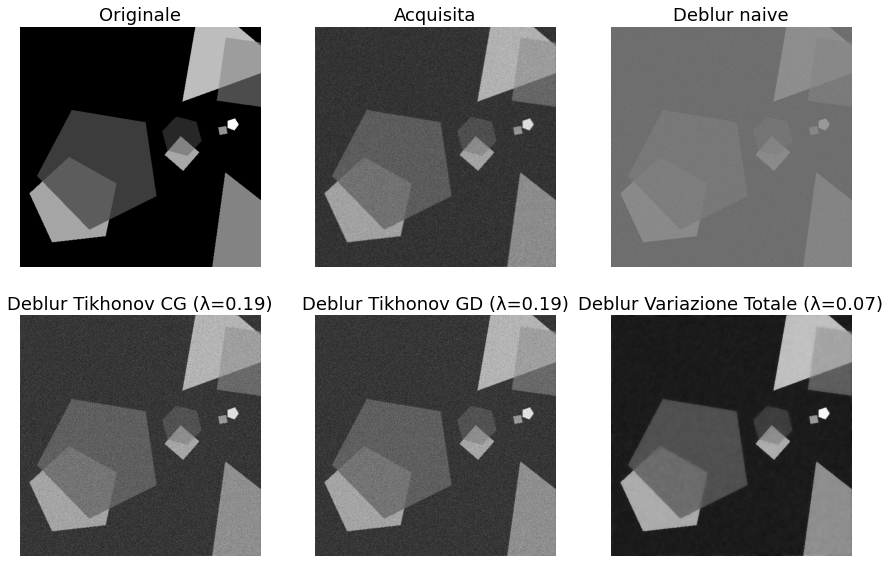
\includegraphics[width=12cm]{esecuzione/1/deblur.png}
    \caption{Risultato del processo di deblur}
    \label{fig:deblur1}
\end{figure}

\begin{center}
    \begin{tabular}{ |c|c|c|c|c|c| }
    \hline
    & Acquisita & Naive & Tikhonov CG & Tikhonov GD & Variazione totale \\ 
    \hline
    MSE & $0.2699 \cdot 10^{-2}$ & $0.2047 \cdot 10^{0}$ & $0.33197 \cdot 10^{-2}$ & $0.3320 \cdot 10^{-2}$ & $0.2119 \cdot 10^{-3}$ \\ 
    PSNR & $25.6878$ & $6.8874$ & $24.7890$ & $24.7890$ & $36.7382$ \\ 
    Iter. & & 140 & 14 & 48 & 14 \\ 
    \hline
    \end{tabular}
\end{center}

Come atteso, la ricostruzione ottenuta con la formulazione come problema ai minimi quadrati senza regolarizzazione ha prodotto un'immagine molto distante dall'originale.\\
Utilizzando la regolarizzazione di Tikhonov, si è ottenuto un risultato quasi invariato rispetto all'immagine acquisita se non addirittura peggiore, mentre, a livello di velocità, il metodo del gradiente ha richiesto più iterazioni rispetto al metodo del gradiente coniugato.\\
Con la regolarizzazione tramite variazione totale, il risultato ottenuto è invece migliore rispetto agli altri metodi e visivamente molto vicina all'immagine originale.\\

\subsection{Seconda esecuzione}
Per vedere le prestazioni di Tikhonov in uno scenario differente, è stata effettuata una seconda esecuzione sulla stessa immagine di partenza con blur ottenuto da un kernel $24 \times 24$ con $\sigma=3$ e rumore con deviazione standard $0.05$.

\subsubsection{Stima di $\lambda$}
\begin{figure}[H]
    \centering
    \begin{minipage}{0.45\textwidth}
        \centering
        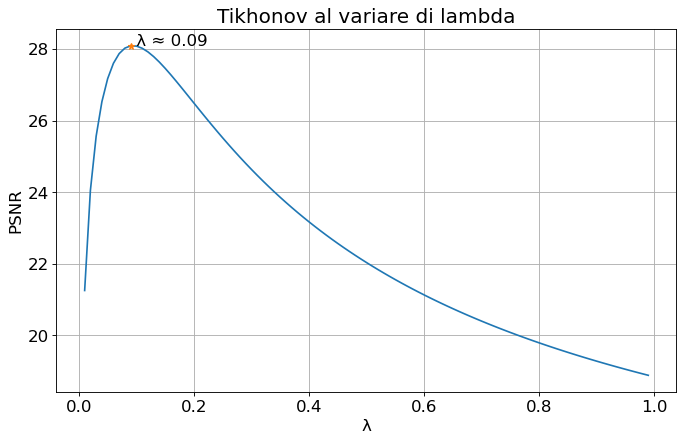
\includegraphics[width=7cm]{esecuzione/2/tikhonov_lambda.png}
        \caption{$\lambda=0.09$ e $\texttt{PSNR} \simeq 28.09$}
        \label{fig:tikhonov_lambda2}
    \end{minipage}\hfill
    \begin{minipage}{0.45\textwidth}
        \centering
        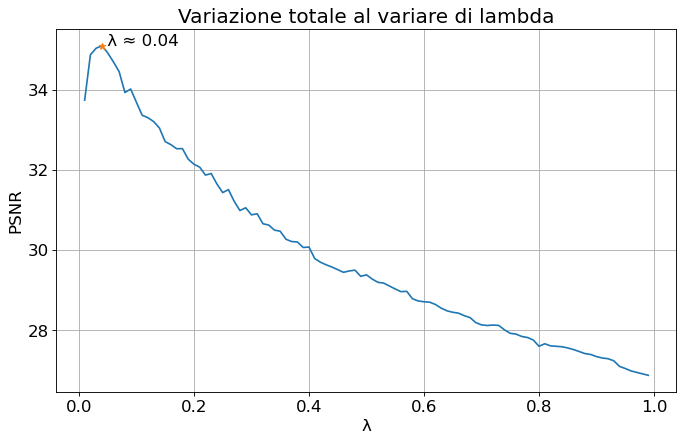
\includegraphics[width=7cm]{esecuzione/2/tv_lambda.png}
        \caption{$\lambda=0.04$ e $\texttt{PSNR} \simeq 35.09$}
        \label{fig:tv_lambda2}
    \end{minipage}
\end{figure}

\subsubsection{Esecuzione}
\begin{figure}[H]
    \centering
    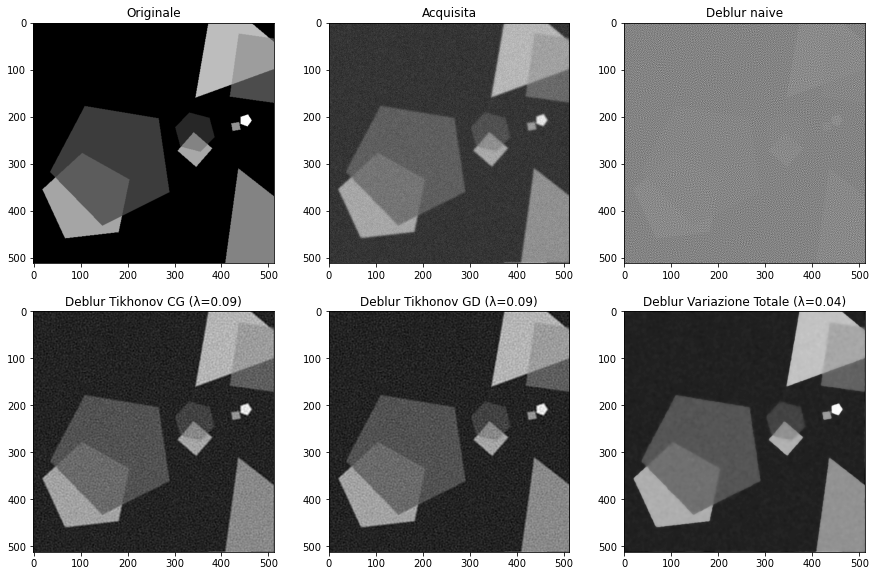
\includegraphics[width=12cm]{esecuzione/2/deblur.png}
    \caption{Risultato del processo di deblur}
    \label{fig:deblur2}
\end{figure}

\begin{center}
    \begin{tabular}{ |c|c|c|c|c|c| }
    \hline
    & Acquisita & Naive & Tikhonov CG & Tikhonov GD & Variazione totale \\ 
    \hline
    MSE & $0.3204 \cdot 10^{-2}$ & $0.5719 \cdot 10^{-1}$ & $0.1553 \cdot 10^{-2}$ & $0.1553 \cdot 10^{-2}$ & $0.3094 \cdot 10^{-3}$ \\ 
    PSNR & $24.9437$ & $-7.5735$ & $28.0889$ & $28.0890$ & $35.0944$ \\ 
    Iter. & & 200 (max) & 18 & 99 & 29 \\ 
    \hline
    \end{tabular}
\end{center}

Anche in questo caso, il metodo naive non ha prodotto soluzioni accettabili, mentre la regolarizzazione tramite variazione totale ha prodotto il risultato migliore.\\
Il metodo regolarizzato con Tikhonov, a differenza dell'esecuzione precedente, ha prodotto un risultato migliore dell'immagine acquisita e, 
analogamente, il numero di iterazioni del metodo che minimizza con il gradiente coniugato è minore rispetto al metodo del gradiente.

\section{Confronto tra gradiente coniugato e metodo del gradiente}
\label{chap:confronto}
Si analizzano ora le prestazioni di Tikhonov utilizzando i due metodi di discesa implementati, focalizzando l'attenzione sulla velocità e precisione. \\

\subsection{Prima esecuzione}
Per una prima sperimentazione si è usata la \autoref{fig:originale1} con kernel $5 \times 5$ con $\sigma=0.5$ e rumore gaussiano con deviazione standard $0.05$.\\
I risultati ottenuti sono i seguenti:
\begin{figure}[H]
    \centering
    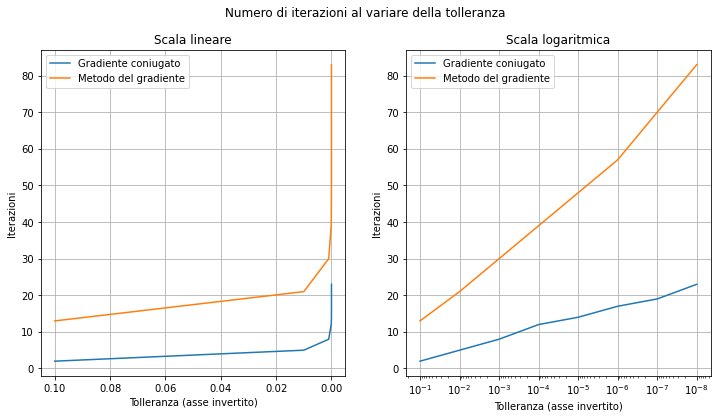
\includegraphics[width=10cm]{iterazioni_cg_gd/1/tol_iter.png}
    \caption{Numero di iterazioni al variare della tolleranza}
    \label{fig:tol_iter1}
\end{figure}
È immediato notare che il metodo del gradiente coniugato necessita di meno iterazioni rispetto al metodo del gradiente prima di raggiungere le condizioni di convergenza.\\

\begin{figure}[H]
    \centering
    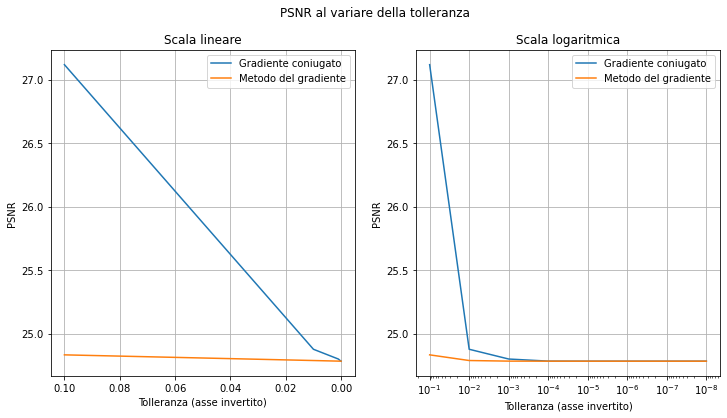
\includegraphics[width=10cm]{iterazioni_cg_gd/1/tol_psnr.png}
    \caption{PSNR al variare della tolleranza}
    \label{fig:tol_psnr1}
\end{figure}
A livello di precisione, il risultato ottenuto mostra che i due metodi, al variare della tolleranza, convergono allo stesso risultato.\\
È però presente un comportamento controintuitivo in vicinanza di valori di tolleranza elevati. 
Infatti si ottiene un PSNR maggiore in corrispondenza di tali valori, in altri termini, si ottiene un'immagine più fedele all'originale con meno iterazioni, mentre il risultato peggiora nella continuazione dell'esecuzione (Tale problematica verrà approfondita nella \autoref{chap:semiconv}).

\begin{figure}[H]
    \centering
    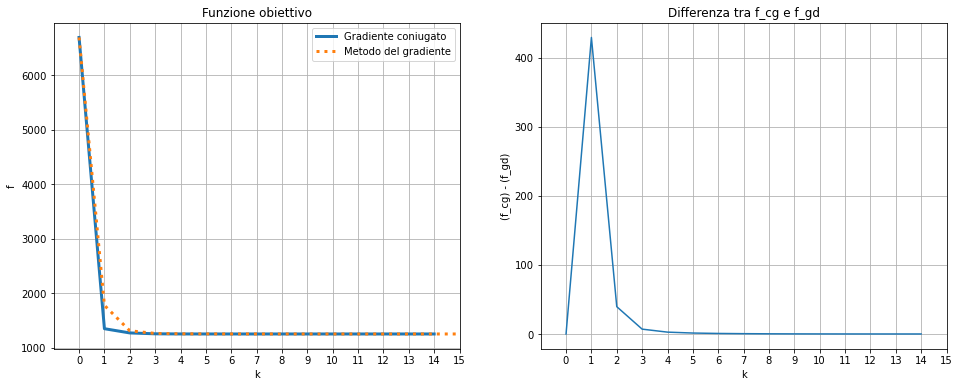
\includegraphics[width=12cm]{iterazioni_cg_gd/1/funzione_obiettivo.png}
    \caption{Andamento della funzione obiettivo}
    \label{fig:obiettivo1}
\end{figure}
\begin{figure}[H]
    \centering
    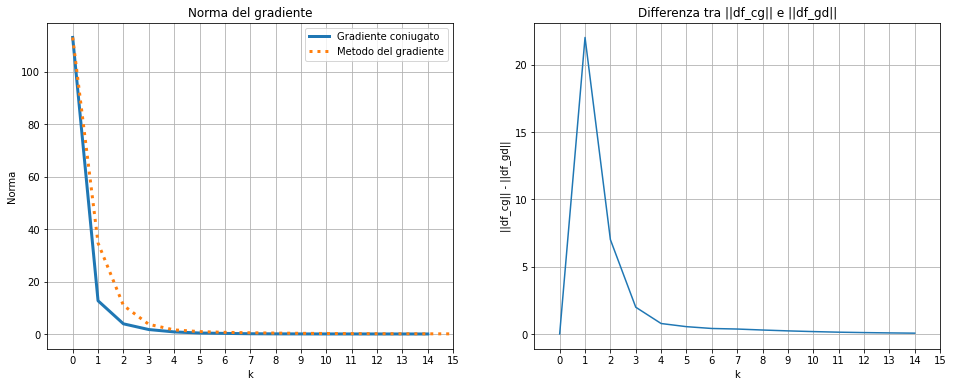
\includegraphics[width=12cm]{iterazioni_cg_gd/1/norma_gradiente.png}
    \caption{Andamento della norma del gradiente}
    \label{fig:gradiente1}
\end{figure}
Infine, come atteso dai risultati precedenti, per il metodo del gradiente coniugato la decrescita della funzione obiettivo è maggiore rispetto al metodo del gradiente. 
Lo stesso risultato è osservabile con la norma del gradente che nel caso del gradiente coniugato esegue passi di dimensione maggiore.

\subsection{Seconda esecuzione}
Per una seconda valutazione si è usato un kernel $24 \times 24$ con $\sigma=3$ e rumore gaussiano con deviazione standard $0.05$.\\

\begin{figure}[H]
    \centering
    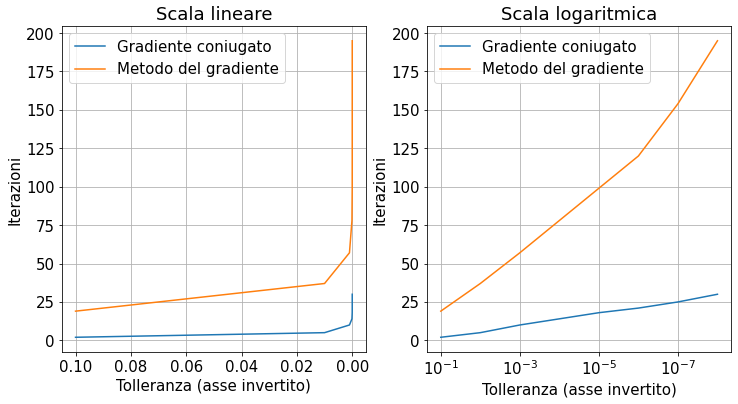
\includegraphics[width=10cm]{iterazioni_cg_gd/2/tol_iter.png}
    \caption{Numero di iterazioni al variare della tolleranza}
    \label{fig:tol_iter2}
\end{figure}
\begin{figure}[H]
    \centering
    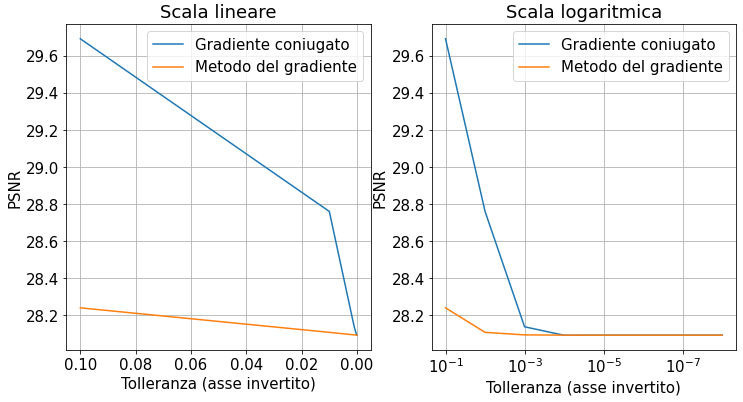
\includegraphics[width=10cm]{iterazioni_cg_gd/2/tol_psnr.png}
    \caption{PSNR al variare della tolleranza}
    \label{fig:tol_psnr2}
\end{figure}
\begin{figure}[H]
    \centering
    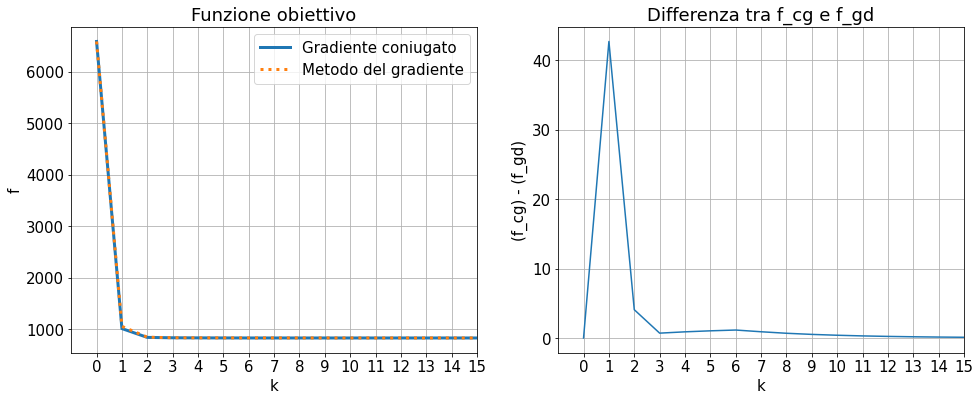
\includegraphics[width=11cm]{iterazioni_cg_gd/2/funzione_obiettivo.png}
    \caption{Andamento della funzione obiettivo}
    \label{fig:obiettivo2}
\end{figure}
\begin{figure}[H]
    \centering
    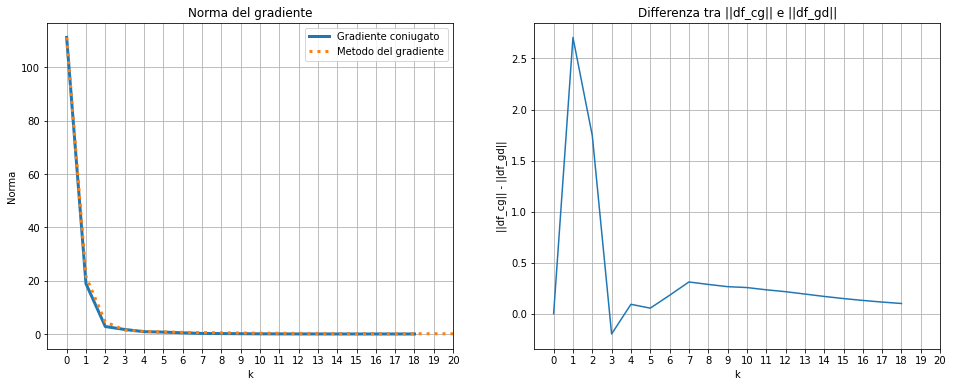
\includegraphics[width=11cm]{iterazioni_cg_gd/2/norma_gradiente.png}
    \caption{Andamento della norma del gradiente}
    \label{fig:gradiente2}
\end{figure}

I risultati ottenuto sono in linea con quelli precedenti ed evidenziano che le prestazioni del gradiente coniugato sono maggiori rispetto a quelle del metodo del gradiente, come atteso dalle analisi teoriche.\\
La soluzione calcolata invece, escludendo valori di tolleranza elevati, converge intorno allo stesso valore e per questo motivo è, in generale, indifferente utilizzare l'implementazione del deblur con i due metodi di discesa. Ovviamente per questioni di velocità, si preferisce utilizzare il metodo implementato con il gradiente coniugato.

\section{Semi-convergenza}
\label{chap:semiconv}
Nella \autoref{chap:confronto} è emerso il problema per cui l'immagine ottenuta con meno iterazioni è migliore rispetto a quella ottenuta quando il metodo raggiunge convergenza. 
Tale problema è noto come semi-convergenza, ovvero quando il raggiungimento dell'ottimo non corrisponde al soddisfacimento delle condizioni di convergenza e per questo le iterazioni successive peggiorano il risultato.\\
Nel contesto del deblur, il problema di semi-convergenza è causato dal rumore aggiunto all'immagine. È noto che il metodo naive è quello che più viene condizionato dal rumore e per questa ragione vengono introdotti i metodi di regolarizzazione.\\
Si analizza quindi il risultato dei vari metodi valutando l'andamento del PSNR rispetto all'iterato $x_{k}$:

\subsection{Analisi con rumore}
\subsubsection{Metodo naive}
\begin{figure}[H]
    \centering
    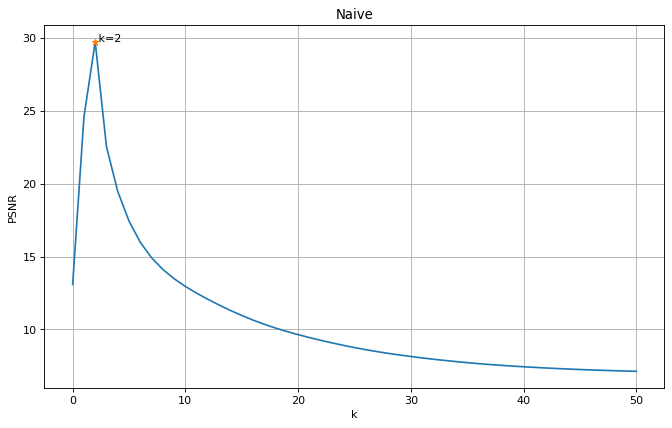
\includegraphics[width=10cm]{semiconvergenza/1/psnr_naive.png}
    \caption{PSNR al variare del numero delle iterazioni}
    \label{fig:semiconv_psnr_naive1}
\end{figure}
\begin{figure}[H]
    \centering
    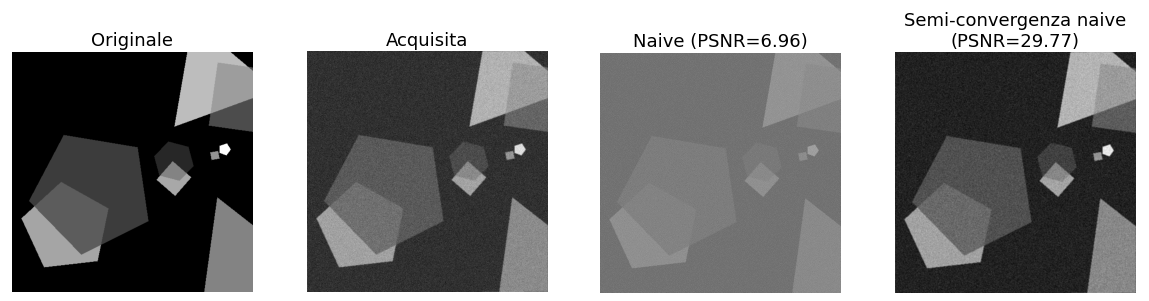
\includegraphics[width=7cm]{semiconvergenza/1/deblur_naive.png}
    \caption{Risultato ottenuto}
    \label{fig:semiconv_deblur_naive1}
\end{figure}
Come atteso, il risultato viene distorto molto rapidamente e non viene raggiunta convergenza nel punto ottimo.

\subsubsection{Regolarizzazione di Tikhonov}
\begin{figure}[H]
    \centering
    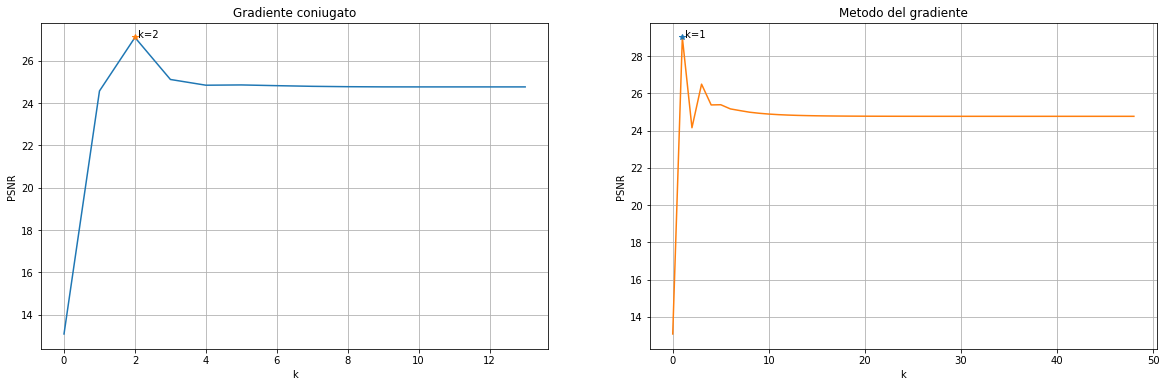
\includegraphics[width=15cm]{semiconvergenza/1/psnr_tikhonov.png}
    \caption{PSNR al variare del numero delle iterazioni}
    \label{fig:semiconv_psnr_tikhonov1}
\end{figure}
\begin{figure}[H]
    \centering
    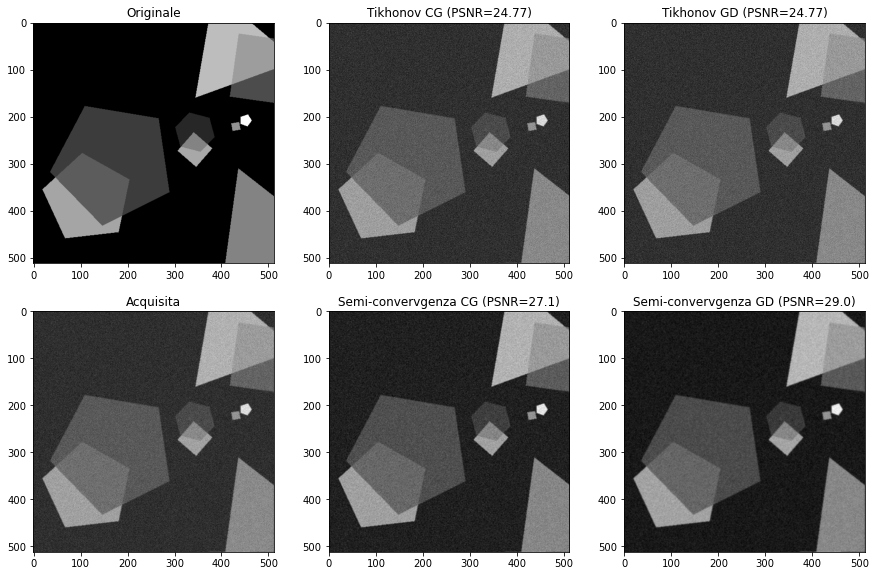
\includegraphics[width=10cm]{semiconvergenza/1/deblur_tikhonov.png}
    \caption{Risultato ottenuto}
    \label{fig:semiconv_deblur_tikhonov1}
\end{figure}
La regolarizzazione di Tikhonov viene introdotta per ridurre l'impatto del rumore sul risultato finale. 
Infatti si nota che, nonostante sia ancora presente il problema di semi-convergenza, dopo il punto di ottimo l'errore decresce di una quantità più contenuta rispetto al metodo naive fino ad assumere un comportamento asintotico.

\subsubsection{Regolarizzazione tramite variazione totale}
\begin{figure}[H]
    \centering
    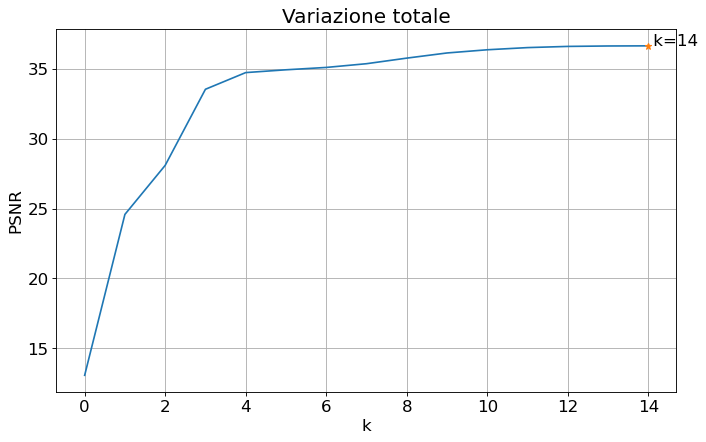
\includegraphics[width=10cm]{semiconvergenza/1/psnr_tv.png}
    \caption{PSNR al variare del numero delle iterazioni}
    \label{fig:semiconv_psnr_tv1}
\end{figure}
\begin{figure}[H]
    \centering
    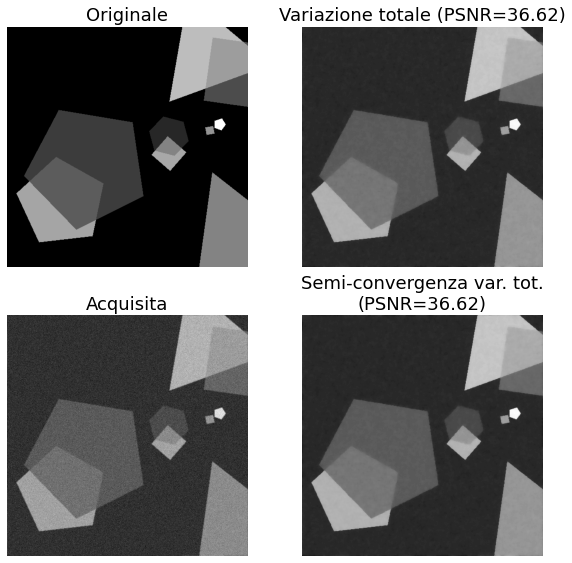
\includegraphics[width=8cm]{semiconvergenza/1/deblur_tv.png}
    \caption{Risultato ottenuto}
    \label{fig:semiconv_deblur_tv1}
\end{figure}
Regolarizzando tramite variazione totale invece, il problema di semi-convergenza è assente nel caso dell'immagine analizzata e il raggiungimento dell'ottimo avviene contemporaneamente al soddisfacimento delle condizioni di convergenza.

\subsubsection{Considerazioni finali}
Le prove precedenti sono state eseguite con kernel $5 \times 5$ con $\sigma=0.5$ e kernel $24 \times 24$ con $\sigma=3$, entrambi i casi con rumore con deviazione standard $0.05$.\\
Nel caso generale, non è possibile risolvere il problema di semi-convergenza interrompendo l'esecuzione quando si rileva un punto di massimo. 
Un controesempio è il caso del metodo del gradiente in \autoref{fig:semiconv_psnr_tikhonov1}, infatti, l'andamento del PSNR può assume più punti di massimo locale e quindi esisteranno casi in cui il primo massimo raggiunto non sarà necessariamente la soluzione ottima.

\subsection{Analisi senza rumore}
Si eseguono ora gli stessi esperimenti su un'immagine a cui è stato applicato un blur senza aggiungere rumore.\\
Un aspetto da tenere in considerazione è che la ricerca del parametro di regolarizzazione $\lambda$ ha prodotto risultati tendenti a 0. Per evitare di annullare il termine di regolarizzazione, riconducendosi al metodo naive, è stato scelto un valore di $\lambda$ molto piccolo.

\begin{figure}[H]
    \centering
    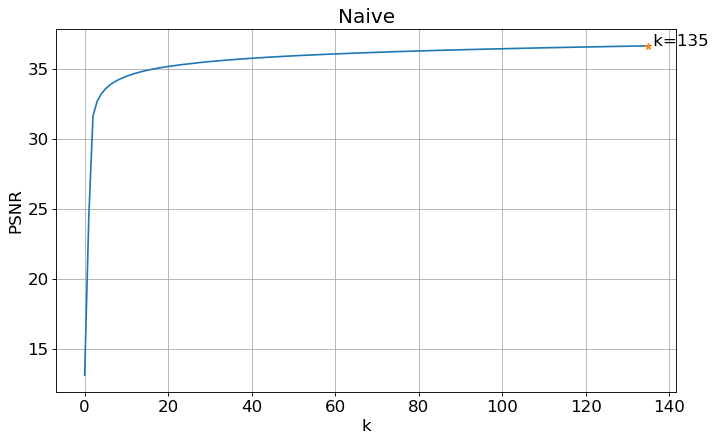
\includegraphics[width=8cm]{semiconvergenza/3/psnr_naive.png}
    \caption{PSNR al variare del numero delle iterazioni con il metodo naive}
    \label{fig:semiconv_psnr_naive3}
\end{figure}
\begin{figure}[H]
    \centering
    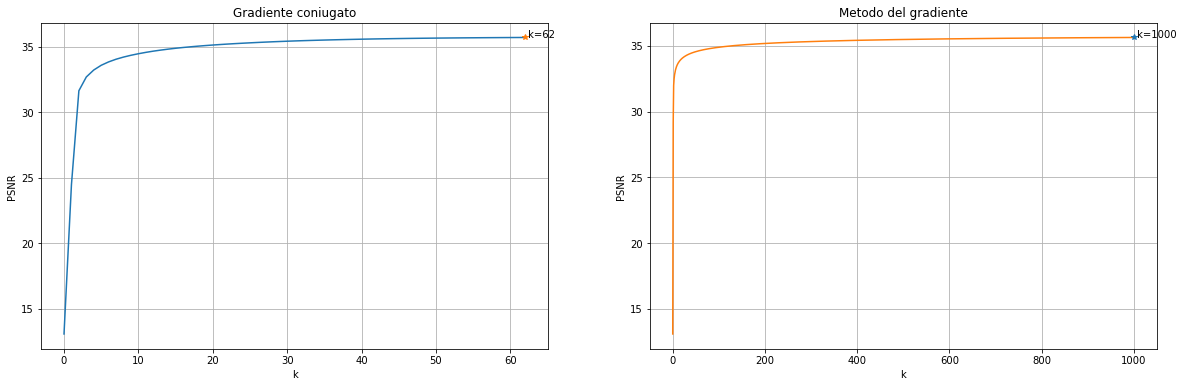
\includegraphics[width=15cm]{semiconvergenza/3/psnr_tikhonov.png}
    \caption{PSNR al variare del numero delle iterazioni con regolarizzazione di Tikhonov}
    \label{fig:semiconv_deblur_tikhonov3}
\end{figure}
\begin{figure}[H]
    \centering
    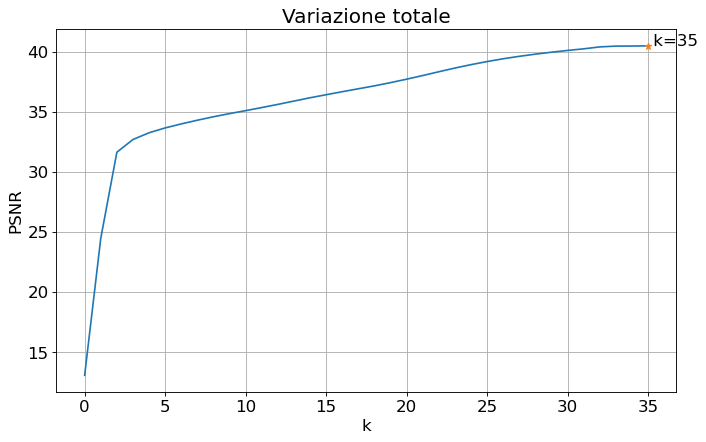
\includegraphics[width=8cm]{semiconvergenza/3/psnr_tv.png}
    \caption{PSNR al variare delle iterazioni con regolarizzazione tramite variazione totale}
    \label{fig:semiconv_deblur_tv3}
\end{figure}
\begin{figure}[H]
    \centering
    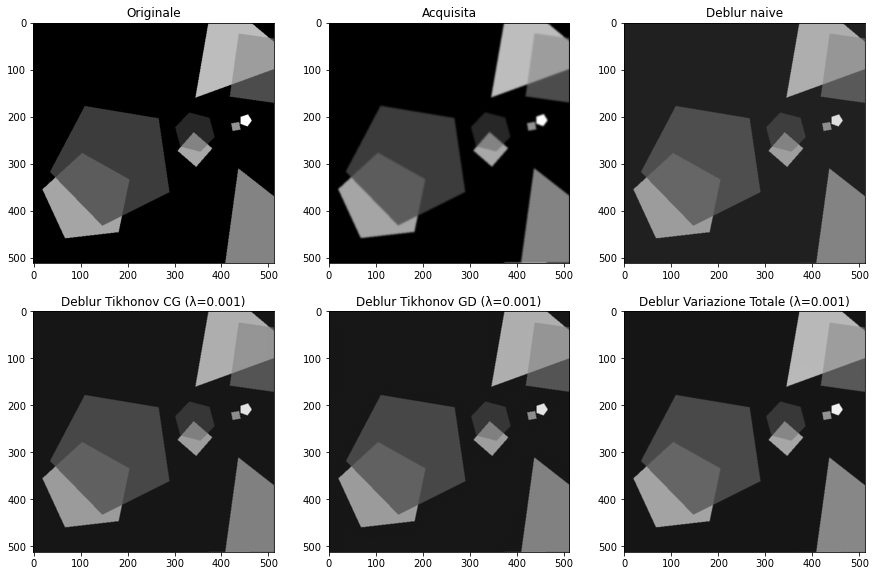
\includegraphics[width=10cm]{semiconvergenza/3/deblur_all.png}
    \caption{Risultato ottenuto}
    \label{fig:semiconv_deblur3}
\end{figure}
Come atteso tutti i metodi hanno raggiunto convergenza e ottimo contemporaneamente e il risultato, in assenza di rumore, si presenta visivamente molto simile indipendentemente dalla formulazione.

\section{Risultati su esecuzioni multiple}
\subsection{Esecuzioni su un dataset generato casualmente}
Per una valutazione complessiva dei metodi, sono stati eseguiti dei test su un dataset di immagini contenenti poligoni regolari generati casualmente 
a cui è stato applicato un blur con kernel $9 \times 9$ con $\sigma_{blur}=1.3$ e rumore con $\sigma_{noise}=0.05$.\\
Come concluso in \autoref{chap:confronto}, verrà utilizzato solamente il metodo del gradiente coniugato poiché produce, in tempo minore, lo stesso risultato del metodo del gradiente.\\
I risultati sono i seguenti:
\begin{figure}[H]
    \centering
    \begin{minipage}{0.45\textwidth}
        \centering
        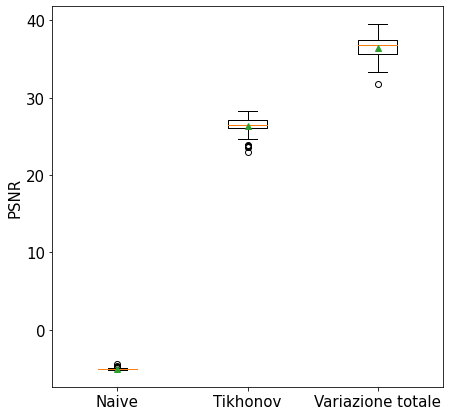
\includegraphics[width=6.5cm]{esecuzioni_multiple/100/psnr1.png}
        \label{fig:100_psnr1}
    \end{minipage}\hfill
    \begin{minipage}{0.45\textwidth}
        \centering
        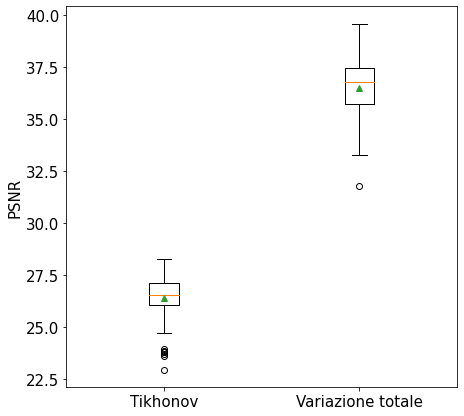
\includegraphics[width=6.5cm]{esecuzioni_multiple/100/psnr2.png}
        \label{fig:100_psnr2}
    \end{minipage}
    \caption{Boxplot al variare del PSNR}
\end{figure}
\begin{center}
    \begin{tabular}{ |c|c|c| }
    \hline
    & Tikhonov & Variazione totale \\ 
    \hline
    Intervallo (\emph{outlier} esclusi) & $[26.03, 28.25]$ & $[35.71, 39.58]$ \\
    Media & $26.39$ & $36.49$ \\
    Mediana & $26.53$ & $36.76$ \\
    Deviazione standard & $1.05$ & $1.38$ \\
    \hline
    \end{tabular}
\end{center}
In linea con i risultati precedenti, il metodo naive ha prodotto soluzioni non accettabili, 
mentre i metodi regolarizzati hanno un comportamento migliore ed è evidente che i risultati ottenuti regolarizzando con variazione totale sono migliori rispetto a quelli ottenuti con Tikhonov.\\

\begin{figure}[H]
    \centering
    \begin{minipage}{0.45\textwidth}
        \centering
        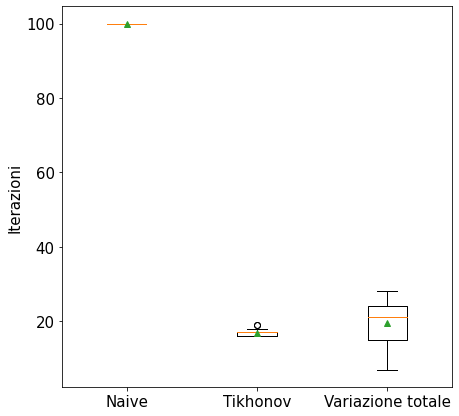
\includegraphics[width=6.5cm]{esecuzioni_multiple/100/iter1.png}
        \label{fig:100_iter1}
    \end{minipage}\hfill
    \begin{minipage}{0.45\textwidth}
        \centering
        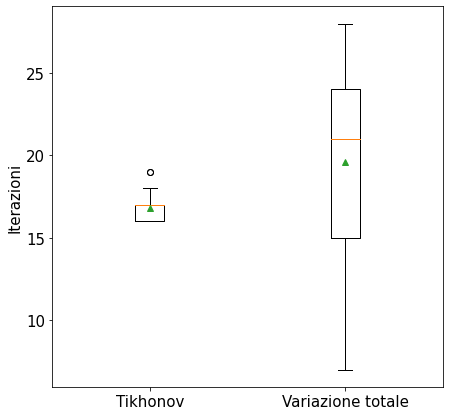
\includegraphics[width=6.5cm]{esecuzioni_multiple/100/iter2.png}
        \label{fig:100_iter2}
    \end{minipage}
    \caption{Boxplot al variare del numero di iterazioni}
\end{figure}

\begin{center}
    \begin{tabular}{ |c|c|c| }
    \hline
    & Tikhonov & Variazione totale \\ 
    \hline
    Intervallo (\emph{outlier} esclusi) & $[16, 18]$ & $[15, 28]$ \\
    Media & $16.79$ & $19.59$ \\
    Mediana & $17$ & $21$ \\
    Deviazione standard & $0.75$ & $5.47$ \\
    \hline
    \end{tabular}
\end{center}
Anche a livello di numero di iterazioni, il metodo naive ha avuto il risultato peggiore, terminando raggiungendo il numero massimo di iterazioni.\\
La regolarizzazione di Tikhonov ha richiesto un numero di iterazioni contentuto e coerente, mentre la regolarizzazione tramite variazione totale ha mostrato dati più diradati e meno prevedibili.\\
In linea di massima, sperimentalmente si è notato che il tempo di esecuzione richiesto con il metodo tramite variazione totale è stato in generale maggiore rispetto a Tikhonov.

\subsection{Esecuzioni sul dataset}
Rispetto al dataset utilizzato, sono state eseguite diverse misurazioni al variare della dimensione del kernel, del valore di $\sigma_{\text{kernel}}$ e della deviazione standard del rumore. 
Per tutte le esecuzioni è stato scelto il valore del parametro di regolarizzazione utilizzando lo stesso procedimento iterativo della \autoref{chap:lambda}.\\
I risultati in forma aggregata sono i seguenti:
\begin{center}
    \begin{tabular}{ |cc|c|c|c|c|c|c|c| }
    \hline
    & & & \multicolumn{3}{c|}{MSE} & \multicolumn{3}{c|}{PSNR} \\
    \hline
    \multicolumn{2}{|c|}{Kernel} & Noise & Naive & Tikhonov & Var. tot. & Naive & Tikhonov & Var. tot. \\ 
    \hline
	$7 \times 7$ & $\sigma=0.5$ & $\sigma=0.05$ & $0.19 \cdot 10^{0}$ & $0.40 \cdot 10^{-2}$ & $0.21 \cdot 10^{-3}$ & 7.14 & 24.16 & 36.94 \\
	$7 \times 7$ & $\sigma=1$ & $\sigma=0.05$ & $0.10 \cdot 10^{1}$ & $0.27 \cdot 10^{-2}$ & $0.24 \cdot 10^{-3}$ & -0.16 & 25.85 & 36.42 \\
    $7 \times 7$ & $\sigma=1.3$ & $\sigma=0.05$ & $0.76 \cdot 10^{0}$ & $0.24 \cdot 10^{-2}$ & $0.26 \cdot 10^{-3}$ & 1.21 & 26.36 & 36.07 \\
    $7 \times 7$ & $\sigma=3$ & $\sigma=0.05$ & $0.12 \cdot 10^{1}$ & $0.17 \cdot 10^{-2}$ & $0.34 \cdot 10^{-3}$ & -0.63 & 27.8 & 34.88 \\
	\hline
    $9 \times 9$ & $\sigma=0.5$ & $\sigma=0.05$ & $0.19 \cdot 10^{0}$ & $0.40 \cdot 10^{-2}$ & $0.21 \cdot 10^{-3}$ & 7.13 & 24.16 & 36.9 \\
	$9 \times 9$ & $\sigma=1$ & $\sigma=0.05$ & $0.10 \cdot 10^{1}$ & $0.27 \cdot 10^{-2}$ & $0.23 \cdot 10^{-3}$ & -0.17 & 25.85 & 36.42 \\
	$9 \times 9$ & $\sigma=1.3$ & $\sigma=0.05$ & $0.76 \cdot 10^{0}$ & $0.24 \cdot 10^{-2}$ & $0.25 \cdot 10^{-3}$ & 1.18 & 26.35 & 36.16 \\
    $9 \times 9$ & $\sigma=3$ & $\sigma=0.05$ & $0.53 \cdot 10^{0}$ & $0.17 \cdot 10^{-2}$ & $0.36 \cdot 10^{-3}$ & 2.73 & 27.77 & 34.68 \\
    \hline
    $24 \times 24$ & $\sigma=0.5$ & $\sigma=0.05$ & $0.42 \cdot 10^{0}$ & $0.37 \cdot 10^{-2}$ & $0.19 \cdot 10^{-3}$ & 3.81 & 24.48 & 37.21 \\
    $24 \times 24$ & $\sigma=1$ & $\sigma=0.05$ & $0.81 \cdot 10^{0}$ & $0.28 \cdot 10^{-2}$ & $0.23 \cdot 10^{-3}$ & 0.92 & 25.65 & 36.45 \\
    $24 \times 24$ & $\sigma=1.3$ & $\sigma=0.05$ & $0.78 \cdot 10^{0}$ & $0.25 \cdot 10^{-2}$ & $0.25 \cdot 10^{-3}$ & 1.09 & 26.21 & 36.16 \\
    $24 \times 24$ & $\sigma=3$ & $\sigma=0.05$ & $0.35 \cdot 10^{0}$ & $0.18 \cdot 10^{-2}$ & $0.35 \cdot 10^{-3}$ & 4.58 & 27.64 & 34.71 \\
    \hline
	$9 \times 9$ & $\sigma=1.3$ & $\sigma=0.1$ & $0.31 \cdot 10^{1}$ & $0.51 \cdot 10^{-2}$ & $0.42 \cdot 10^{-3}$ & -4.87 & 23.07 & 33.85 \\
	$24 \times 24$ & $\sigma=3$ & $\sigma=0.1$ & $0.14 \cdot 10^{1}$ & $0.36 \cdot 10^{-2}$ & $0.53 \cdot 10^{-3}$ & -1.51 & 24.63 & 32.88 \\
    \hline
    \end{tabular}
\end{center}
Come in tutti i casi precedenti, la ricostruzione naive ha prodotto soluzioni completamente distanti dall'immagine reale.\\
Si nota, invece, un fenomeno ricorrente nella precisione di ricostruzione per i metodi regolarizzati all'aumentare di $\sigma_{\text{kernel}}$. Con Tikhonov si la fedeltà della soluzione rispetto all'immagine reale è maggiore all'aumentare di $\sigma_{\text{kernel}}$, mentre per la variazione totale, il fenomeno è inverso, generando una ricostruzione meno accurata.

\begin{center}
    \begin{tabular}{ |cc|c|c|c|c|c|c|c| }
    \hline
    & & & \multicolumn{3}{c|}{MSE} & \multicolumn{3}{c|}{PSNR} \\
    \hline
    \multicolumn{2}{|c|}{Kernel} & Noise & Naive & Tikhonov & Var. tot. & Naive & Tikhonov & Var. tot. \\ 
    \hline
    $9 \times 9$ & $\sigma=0.5$ & $\sigma=0.05$ & $0.19 \cdot 10^{0}$ & $0.40 \cdot 10^{-2}$ & $0.21 \cdot 10^{-3}$ & 7.13 & 24.16 & 36.9 \\
	$9 \times 9$ & $\sigma=1$ & $\sigma=0.05$ & $0.10 \cdot 10^{1}$ & $0.27 \cdot 10^{-2}$ & $0.23 \cdot 10^{-3}$ & -0.17 & 25.85 & 36.42 \\
	$9 \times 9$ & $\sigma=1.3$ & $\sigma=0.05$ & $0.76 \cdot 10^{0}$ & $0.24 \cdot 10^{-2}$ & $0.25 \cdot 10^{-3}$ & 1.18 & 26.35 & 36.16 \\
    $9 \times 9$ & $\sigma=3$ & $\sigma=0.05$ & $0.53 \cdot 10^{0}$ & $0.17 \cdot 10^{-2}$ & $0.36 \cdot 10^{-3}$ & 2.73 & 27.77 & 34.68 \\
    $9 \times 9$ & $\sigma=4$ & $\sigma=0.05$ & $0.12 \cdot 10^{1}$ & $0.16 \cdot 10^{-2}$ & $0.39 \cdot 10^{-3}$ & -0.79 & 28.14 & 34.24 \\
    $9 \times 9$ & $\sigma=5$ & $\sigma=0.05$ & $0.12 \cdot 10^{1}$ & $0.15 \cdot 10^{-2}$ & $0.42 \cdot 10^{-3}$ & -0.91 & 28.31 & 33.85 \\
    $9 \times 9$ & $\sigma=10$ & $\sigma=0.05$ & $0.85 \cdot 10^{0}$ & $0.17 \cdot 10^{-2}$ & $0.58 \cdot 10^{-3}$ & 0.72 & 27.97 & 32.55 \\
    $9 \times 9$ & $\sigma=15$ & $\sigma=0.05$ & $0.99 \cdot 10^{0}$ & $0.18 \cdot 10^{-2}$ & $0.58 \cdot 10^{-3}$ & 0.06 & 27.71 & 32.52 \\
    $9 \times 9$ & $\sigma=30$ & $\sigma=0.05$ & $0.14 \cdot 10^{1}$ & $0.19 \cdot 10^{-2}$ & $0.59 \cdot 10^{-3}$ & -1.55 & 27.36 & 32.43 \\
    $9 \times 9$ & $\sigma=60$ & $\sigma=0.05$ & $0.16 \cdot 10^{1}$ & $0.20 \cdot 10^{-2}$ & $0.64 \cdot 10^{-3}$ & -2.12 & 27.19 & 32.1 \\
    $9 \times 9$ & $\sigma=100$ & $\sigma=0.05$ & $0.17 \cdot 10^{1}$ & $0.21 \cdot 10^{-2}$ & $0.59 \cdot 10^{-3}$ & -2.29 & 27.08 & 32.42 \\
	$9 \times 9$ & $\sigma=200$ & $\sigma=0.05$ & $0.17 \cdot 10^{1}$ & $0.21 \cdot 10^{-2}$ & $0.61 \cdot 10^{-3}$ & -2.38 & 27.04 & 32.29 \\
	\hline
    \end{tabular}
\end{center}

\end{document}
